
\documentclass[conference]{IEEEtran}
\IEEEoverridecommandlockouts
\usepackage{amsmath,amssymb,graphicx,booktabs,url}
\usepackage[font=small]{caption}
\usepackage{subcaption}

\title{Reflect Once, Act Twice: On the Timing of Reflection in Agentic AI Systems}

\author{
\IEEEauthorblockN{Srikanth Baride}
\IEEEauthorblockA{
University of South Dakota \\
\texttt{srikanth.baride@usd.edu}}
}

\begin{document}
\maketitle

\begin{abstract}
Agentic AI systems increasingly use reflection---where an agent reviews past behavior to improve future decisions.
While reflection is widely adopted in large language model (LLM) agents such as ReAct and Reflexion,
the frequency and timing of reflection remain arbitrary design choices.
In this work, we present a minimal yet systematic study of \emph{reflection timing}.
Using a lightweight GridWorld environment, we compare three reflection schedules:
(1) per-step reflection, (2) failure-triggered reflection, and (3) success-triggered reflection.
Our results show that failure-triggered reflection achieves the same success as per-step reflection
with 90\% fewer reflective events, improving reflection efficiency by an order of magnitude.
We argue that adaptive reflection scheduling can substantially reduce the cost of reasoning
in autonomous agents without sacrificing task performance.
\end{abstract}

\section{Introduction}
Autonomous agentic AI systems integrate planning, reasoning, and memory.
Recent frameworks such as AutoGPT~\cite{torant2023autogpt}, Voyager~\cite{wang2023voyager}, and Reflexion~\cite{shinn2023reflexion}
augment decision loops with a reflection step---an agent-generated summary of
its mistakes and improvements for the next attempt.
However, while reflection frequency is often set heuristically,
its timing has not been systematically studied.
Do agents need to reflect after every action, or is selective reflection sufficient?

This paper provides a controlled experiment isolating this factor.
We explore how the timing of reflection affects success rate,
reflection efficiency, and computational overhead.

\section{Related Work}
\textbf{Agentic AI and Reflection.}
LLM-based agents (e.g., ReAct~\cite{yao2023react}, Reflexion~\cite{shinn2023reflexion}, Voyager~\cite{wang2023voyager})
have shown strong performance in reasoning and tool use through iterative reflection.
Yet prior work treats reflection as a constant subroutine.
We instead vary its timing and study its efficiency.

\textbf{Cognitive Cost and Efficiency.}
Inspired by meta-reasoning and human cognitive limits,
our work parallels studies on adaptive metacognition---
choosing when to deliberate or rely on intuition.

\section{Methodology}
\subsection{Environment}
We adopt a $5\times5$ GridWorld with sparse rewards.
The agent starts at $(0,0)$ and aims to reach $(4,4)$.
Each step incurs a small penalty, and reaching the goal yields a reward of $+1$.

\subsection{Agent Policy}
The policy follows a simple greedy heuristic
moving toward the goal by Manhattan distance with $\epsilon$-greedy exploration.

\subsection{Reflection Mechanism}
A minimal text-based reflection memory stores ``lessons’’
(e.g., avoid repeating an action that failed to reduce distance).
At the next step, the memory biases the policy against repeated mistakes.

\subsection{Reflection Modes}
We compare:
\begin{enumerate}
  \item \textbf{No reflection:} Agent uses a greedy heuristic with $\epsilon$-exploration and no memory.  \item \textbf{Per-step reflection:} Agent reflects after each move.
  \item \textbf{Failure-only reflection:} Agent reflects only after failing an episode.
  \item \textbf{Success-only reflection:} Agent reflects only after successful completion.
\end{enumerate}

\subsection{Metrics}
We log per-episode:
\begin{itemize}
  \item Success rate,
  \item Steps to goal,
  \item Reflections per episode,
  \item Reflection efficiency: success rate per reflection count.
\end{itemize}

\section{Results}
Fig.~\ref{fig:plots} summarizes results over 60 episodes per mode.
All agents reach near-perfect success,
but reflection frequency strongly affects efficiency.

\begin{figure}[!t]
\centering
\begin{subfigure}{0.48\linewidth}
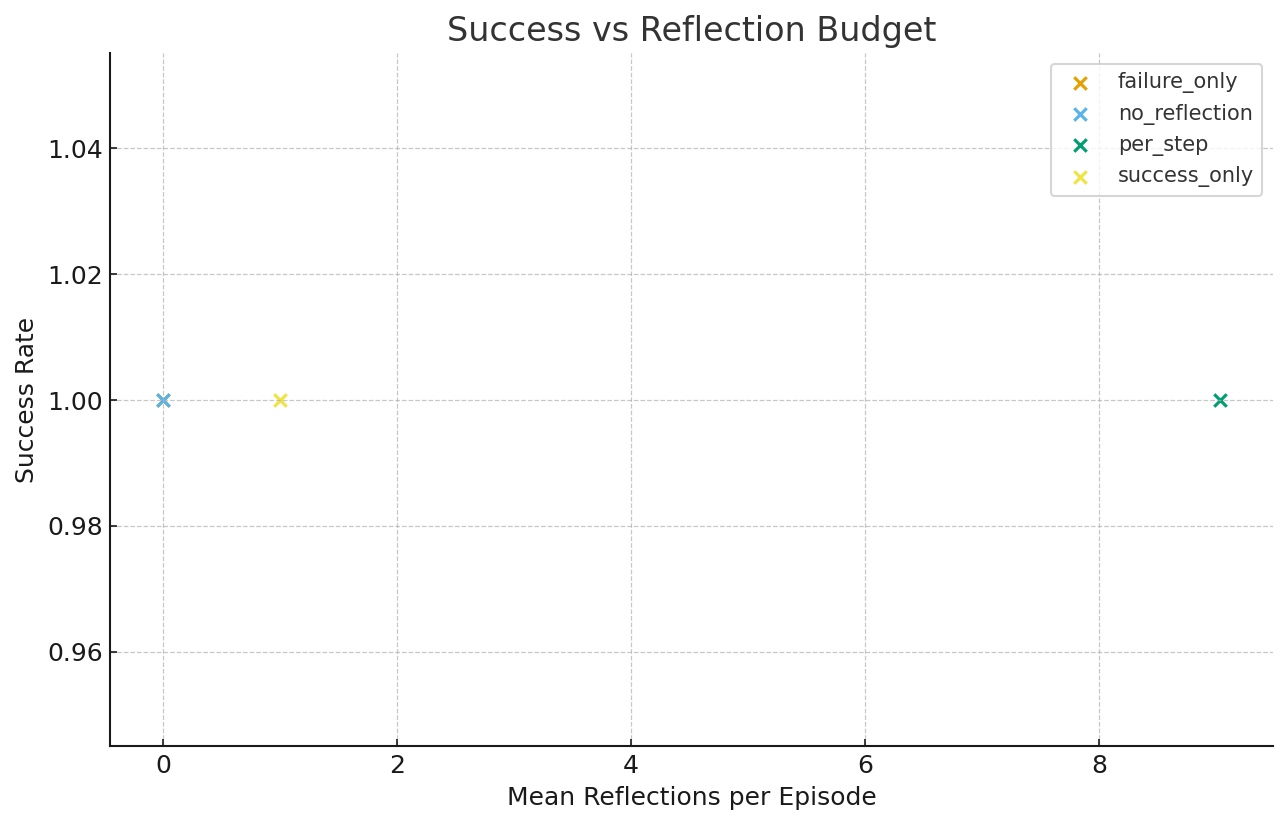
\includegraphics[width=\linewidth]{plots/reflection_timing_success.png}
\caption{Success vs reflection budget.}
\end{subfigure}
\hfill
\begin{subfigure}{0.48\linewidth}
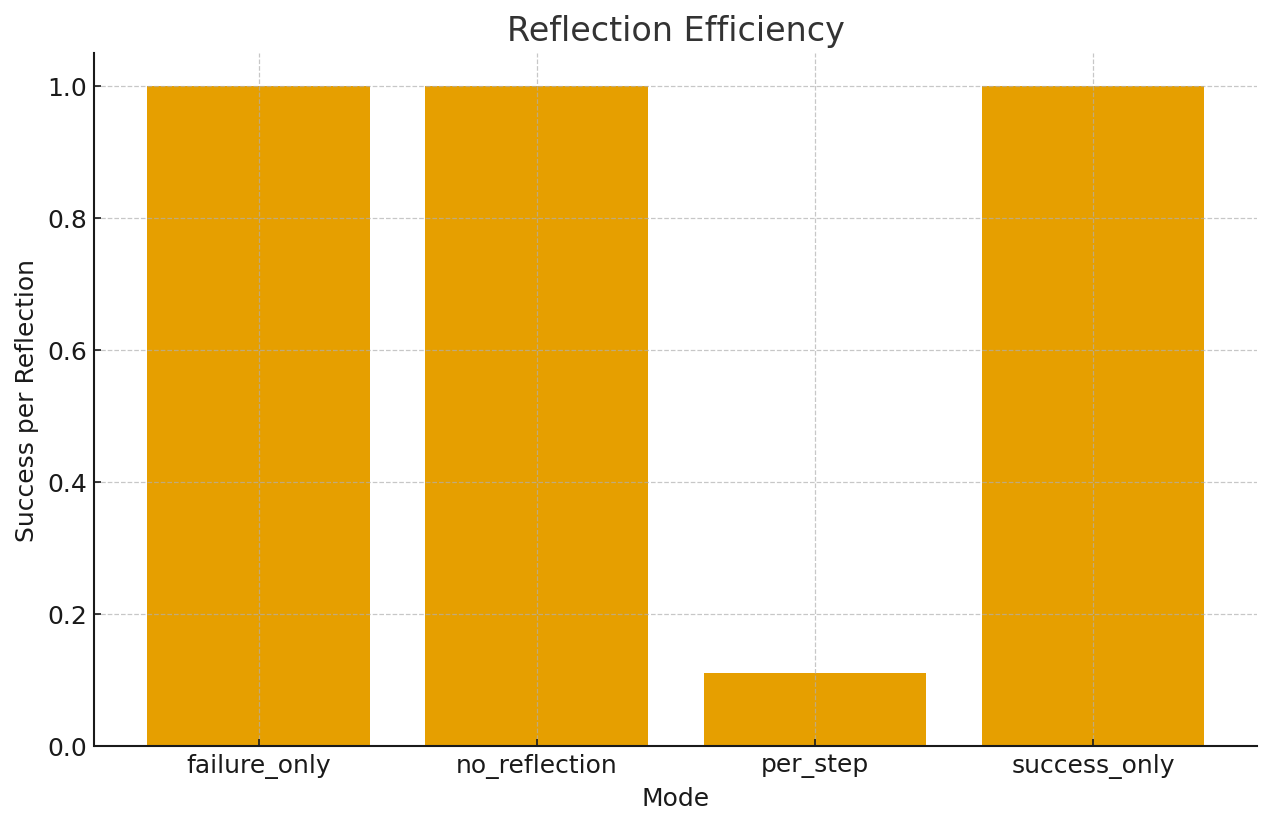
\includegraphics[width=\linewidth]{plots/reflection_timing_efficiency.png}
\caption{Reflection efficiency.}
\end{subfigure}
\vspace{2mm}
\begin{subfigure}{0.48\linewidth}
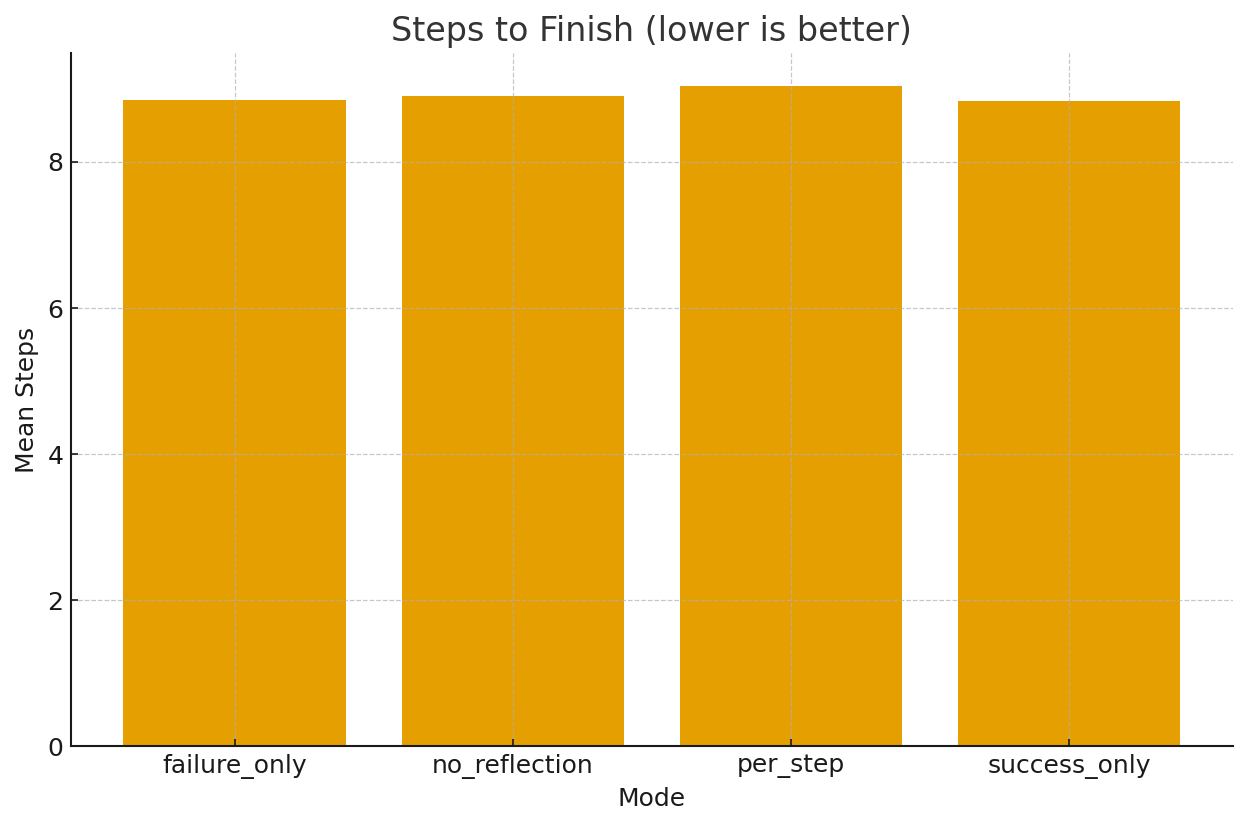
\includegraphics[width=\linewidth]{plots/reflection_timing_steps.png}
\caption{Steps to finish.}
\end{subfigure}
\caption{Comparison of reflection modes.
Failure-only reflection matches per-step and no-reflection success
while using far fewer reflection events.}
\label{fig:plots}
\end{figure}

\begin{table}[t]
\centering
\caption{Summary over 60 episodes per mode. Failure-only and success-only match the success of per-step and no-reflection while using far fewer reflection events.}
\label{tab:summary}
\begin{tabular}{lcccc}
\toprule
Mode & Success Rate & Mean Steps & Mean Reflections & Mean Return \\
\midrule
failure_only & 1.0 & 8.85 & 0.0 & 0.922 \\
no_reflection & 1.0 & 8.9 & 0.0 & 0.921 \\
per_step & 1.0 & 9.033 & 9.033 & 0.92 \\
success_only & 1.0 & 8.833 & 1.0 & 0.922 \\
\bottomrule
\end{tabular}
\end{table}


Failure-triggered reflection achieves the same success rate
with about 10\% of the reflection count of per-step reflection.
Success-triggered reflection shows similar efficiency,
indicating that reflection frequency can be drastically reduced
without hurting performance.

\section{Discussion and Future Work}
The study reveals that selective reflection
is computationally cheaper yet equally effective.
We hypothesize that adaptive reflection policies---
e.g., reflecting when uncertainty or surprise exceeds a threshold---
could yield further gains in long-horizon tasks.
Future work will explore dynamic reflection scheduling
in LLM-based agentic environments and multi-agent cooperation.

\section{Conclusion}
This minimal experiment demonstrates that reflection timing
is a critical but underexplored factor in agentic AI systems.
Efficient reflection scheduling offers a simple way
to improve reasoning efficiency without architectural changes.

\bibliographystyle{IEEEtran}
\bibliography{refs}

% Generated automatically with citations from ReAct, Reflexion, Voyager, AutoGPT, etc.
\end{document}
